


%----------------------------------------------------------------------------------------

\newpage

%%%%%%%%%%%%%%%%%%%%%%%
\section{Fieldwork Elements}{Élements de terrain}
% idem case studies

\label{app:sec:qualitative}
% \label{app:sec:fieldwork}



%%%%%%%%%%%%%%%%%%%%%
\subsection{Fieldwork in China}{Localisation des terrains en Chine}


Nous précisons la localisation géographique des territoires et lieux évoqués en~\ref{sec:casestudies} et en~\ref{sec:qualitative} dans les cartes suivantes. Nous donnons :
\begin{itemize}
	\item Une carte en Fig.~\ref{fig:app:casestudies:nanfang} à l'échelle du sud de la Chine, qui permet de localiser le Delta de la Rivière des Perles (qui inclut Guangzhou et Zhuhai), Chengdu et Leshan, ainsi que Yangshuo.
	\item Une carte en Fig.~\ref{fig:app:casestudies:prd} à l'échelle du Delta de la Rivière des Perles, qui permet de localiser les principales villes : Guangzhou/Foshan, Dongguan, Zhongshan, Zhuhai et Shenzhen (ZES), ainsi que Hong-Kong et Macao (ZAS).
	\item Une carte en Fig.~\ref{fig:app:casestudies:zhuhai} à l'échelle de Zhuhai, qui permet de localiser les différents quartiers de Zhuhai : Gongbei, Xiangzhou, Tangjia, ainsi que la gare de Zhuhai Bei, le pont HZMB et les \emph{New Territories} à Hong-Kong (nous désignons par quartier ici non pas des districts administratifs, puisque par exemple Tangjia fait partie du district de Xinwan, mais des quartiers vécus).
\end{itemize}



%%%%%%%%%%%%%%
\begin{figure}
	%\includegraphics[width=\linewidth]{Figures/CaseStudies/nanfang.png}	
	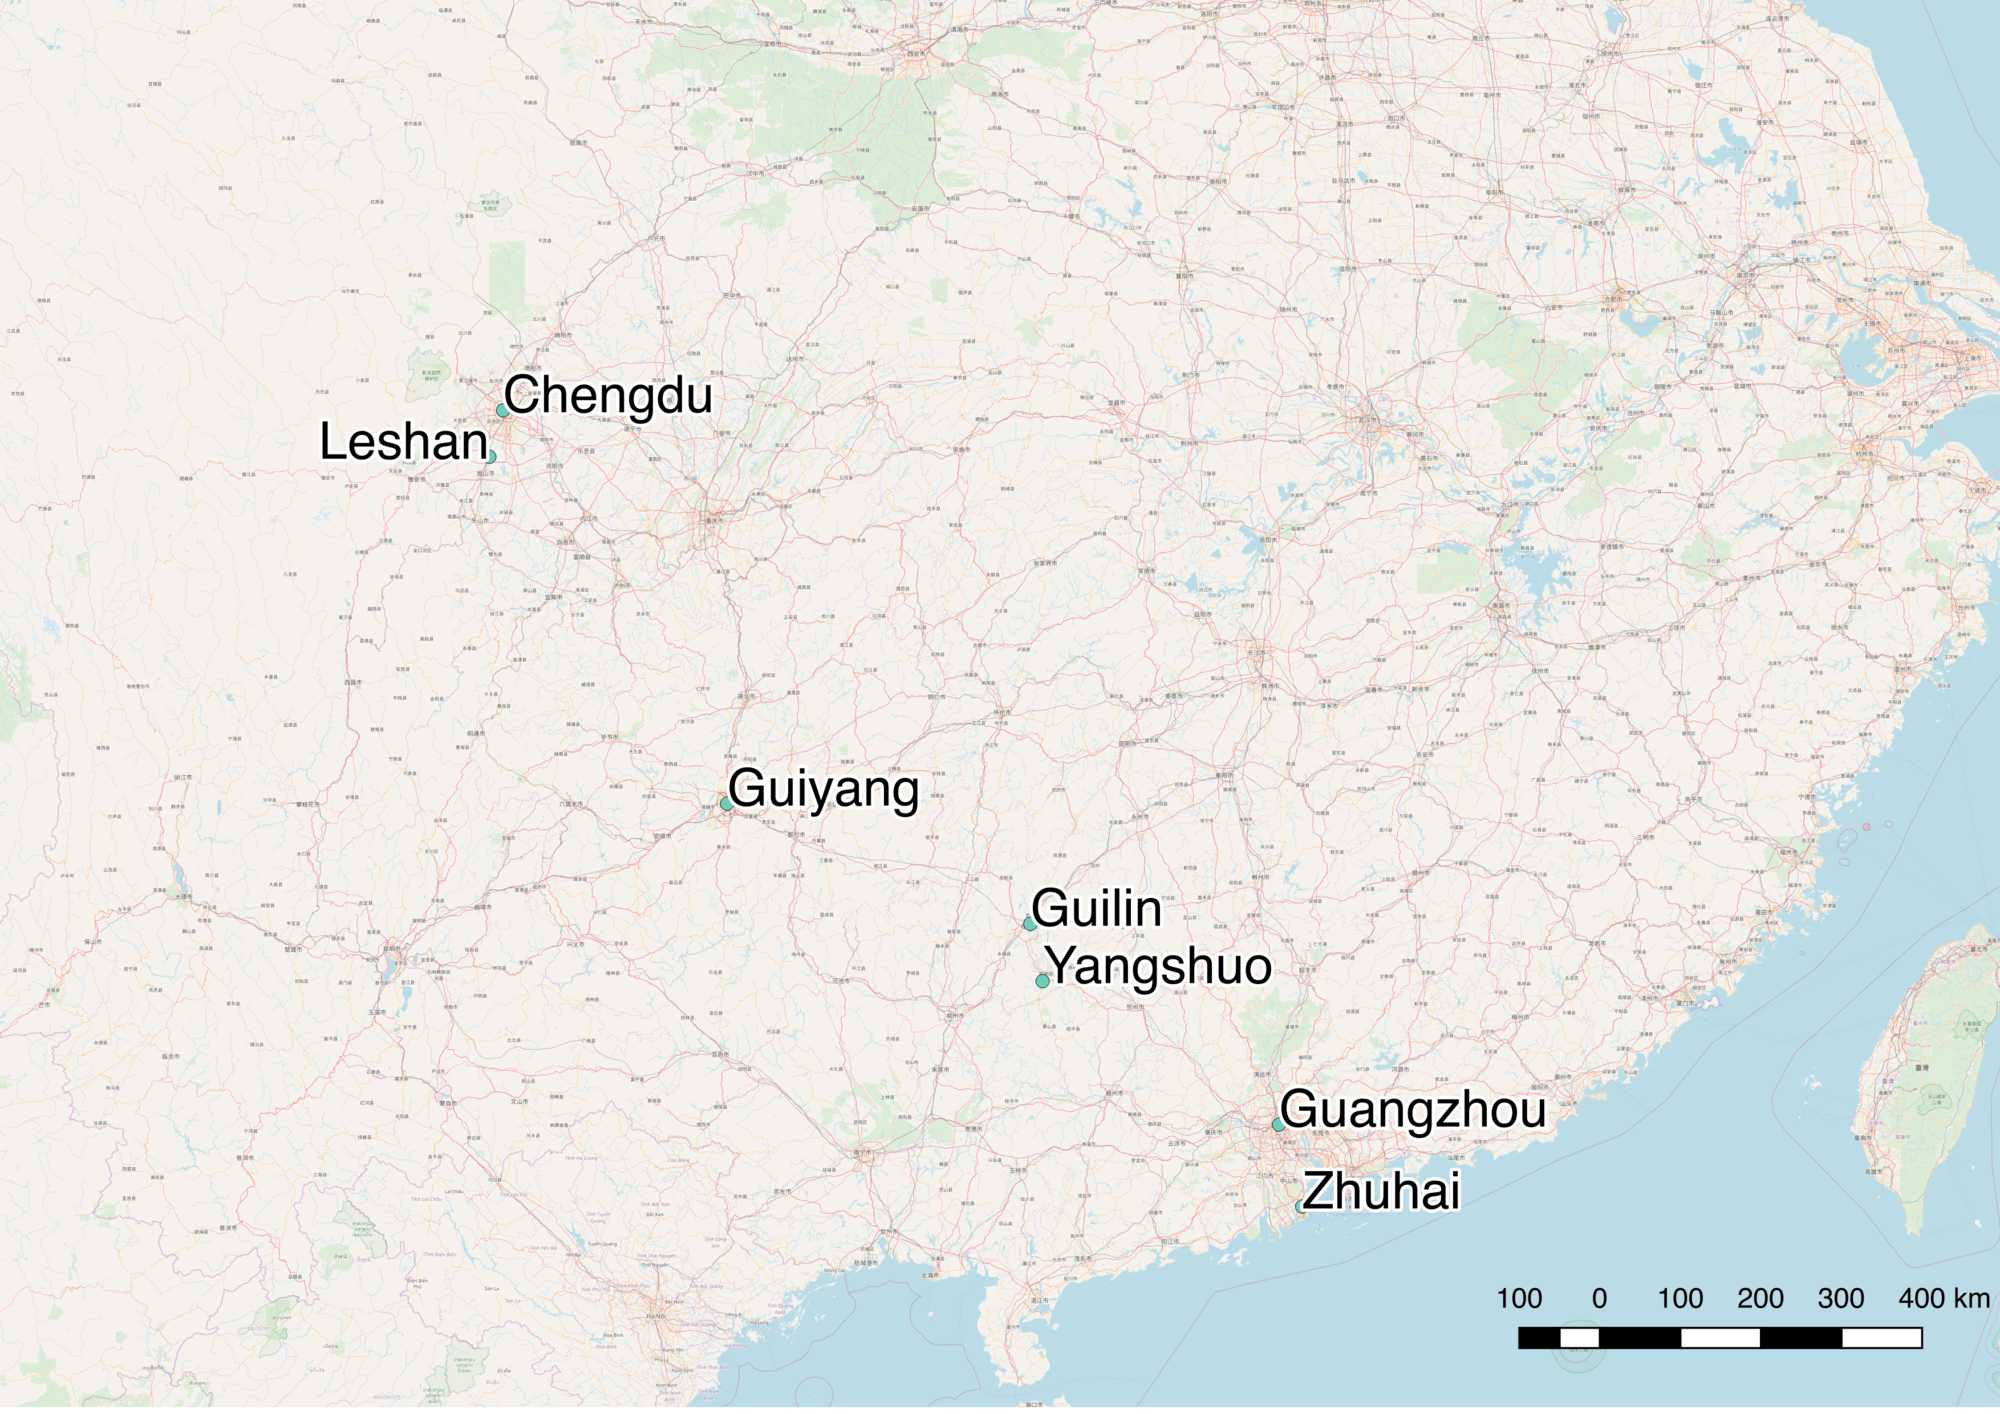
\includegraphics[width=\linewidth]{Figures/Final/A-casestudies-nanfang.jpg}	
	\appcaption{\label{fig:app:casestudies:nanfang}}{\textbf{Localisation des lieux de terrain, } à l'échelle du sud de la Chine. Source : OpenStreetMap.\label{fig:app:casestudies:nanfang}}
\end{figure}
%%%%%%%%%%%%%%


%%%%%%%%%%%%%%
\begin{figure}
	%\includegraphics[width=\linewidth]{Figures/CaseStudies/prd.png}	
	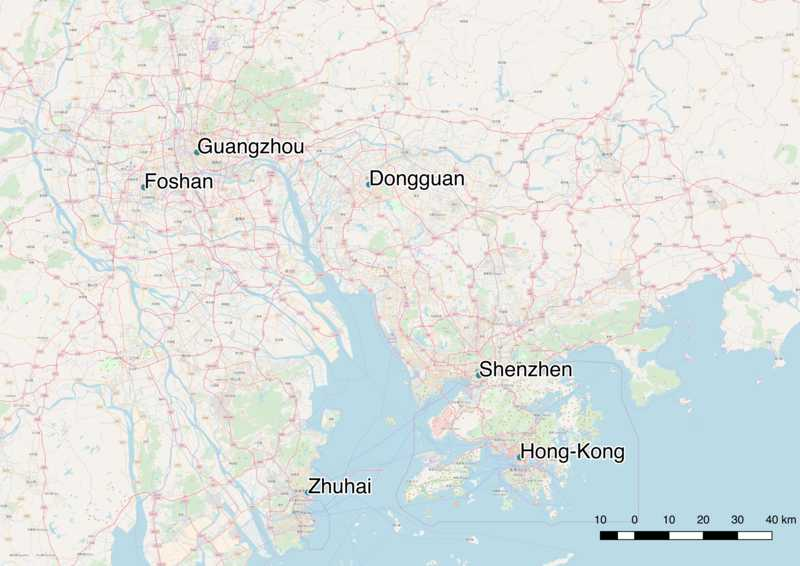
\includegraphics[width=\linewidth]{Figures/Final/A-casestudies-prd.jpg}	
	\appcaption{\label{fig:app:casestudies:prd}}{\textbf{Localisation des lieux de terrain, } à l'échelle du Delta de la Rivière des Perles. Source : OpenStreetMap.\label{fig:app:casestudies:prd}}
\end{figure}
%%%%%%%%%%%%%%


%%%%%%%%%%%%%%
\begin{figure}
	%\includegraphics[width=\linewidth]{Figures/CaseStudies/zhuhai.png}	
	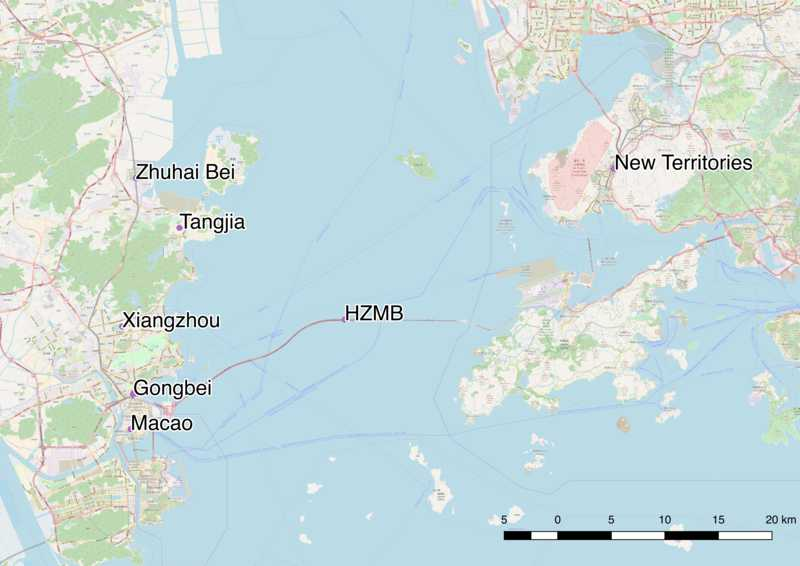
\includegraphics[width=\linewidth]{Figures/Final/A-casestudies-zhuhai.jpg}	
	\appcaption{\label{fig:app:casestudies:zhuhai}}{\textbf{Localisation des lieux étudiés, } à l'échelle de Zhuhai. Source : OpenStreetMap.\label{fig:app:casestudies:zhuhai}}
\end{figure}
%%%%%%%%%%%%%%




%----------------------------------------------------------------------------------------


%%%%%%%%%%%%%%%%%%%%%
\subsection{Fieldwork Notebook}{Carnet de Terrain}

Nous rendons compte ici de manière synthétique les différentes sorties de terrain alimentant la section~\ref{sec:qualitative}. S'il n'est a priori pas standard de fournir de manière brute et ouverte le contenu des carnets de terrain, \cite{goffman1989fieldwork} souligne que celui-ci peut être un matériau de recherche en lui-même. Les compte-rendus bruts et les photos sont disponibles de manière ouverte à \url{https://github.com/JusteRaimbault/CityNetwork/tree/master/Data/Fieldwork}.


Ci-dessous sont résumés les contextes et observations principaux des sorties. Les lieux sont localisés dans les cartes de Fig.~\ref{fig:app:casestudies:nanfang} à Fig.~\ref{fig:app:casestudies:zhuhai}. Les sorties sont effectuées seul sauf si précisé pour certaines d'entre elles.

%%%% 
% -- from redac 01/09 --
% Zhuhai-guangzhou pour aller à HK : train de nuit utilisé pour soirée en mode assis : optimisation des missions.




\paragraph{29/10/2016}{29/10/2016}

Sortie à Zhuhai (Xiangzhou et Gongbei), avec C. Losavio pour guide et interprétation. Nature en ville et utilisation des parcs par les habitants.


\paragraph{06/11/2016}{06/11/2016}

Sortie à Macao par Gongbei, avec C. Losavio. Flux journaliers par la frontière de la ZAS.
% le 5 exactement pour l``interview''.


\paragraph{07/11/2016}{07/11/2016}

Aller-retour Zhuhai-Hong-Kong. Relation apparente des habitants de Zhuhai à la ZAS.

\paragraph{16/01/2017}{16/01/2017}

Tentative de relier Tangjia à Guangzhou par bus de ville, journée. Itinéraire final Tangjia-Zhongshan-Xiaolan-Zhuahaibei. Transports locaux et franges urbaines.


\paragraph{11/12/2016}{11/12/2016}

De Pekin à Shenzhen par Guangzhou et Dongguan. Transports, difficultés d'accessibilité.


\paragraph{8/06/2017}{8/06/2017}

De Hong-Kong à Tangjia par Zhuhai. Transports.


\paragraph{19/06/2017}{19/06/2017}

Visite de terrain officielle dans le cadre de la Conférence Medium, Guangzhou, encadrée par guides et interprètes engagés par l'université SYSU. Rénovation Urbaine, projets urbains, patrimoine.


\paragraph{09/07/2017}{09/07/2017}

Visite des New Territories à Hong-Kong : transport lourd depuis Kwoloon puis différentes lignes de tramway sur place. Retour par le métro de Shenzhen puis par ferry jusqu'à Zhuhai. 


\paragraph{11/07/2017}{11/07/2017}

Aller-retour Tangjia-Guangzhou. Congestion des transports (routier et vélos libre-service).


\paragraph{24/07/2017}{24/07/2017}


Sortie à Tangjia. Discontinuités socio-économiques locales.


\paragraph{31/07/2017}{31/07/2017}

Sortie à Xiangzhou. Test du Tramway, Ligne 2.



\paragraph{09/08/2017}{09/08/2017}

Sortie à Xiangzhou puis Tangjia. Opération de TOD : terminus ouest Tram ; bus pour la gare de Tangjia le long de la ligne à grande vitesse.


\paragraph{13/08/2017}{13/08/2017}

De Yangshuo (Guanxi) à GuangzhouNan par le Train à Grande Vitesse.




\paragraph{17/08/2017}{17/08/2017}


Bureau du Comité de Planification de la zone High Tech de Zhuhai. Administration et bureaucratie.



\paragraph{20/08/2017}{20/08/2017}

Traversée de Leshan (Sichuan) en bus, aller-retour. Transports et Tourisme.



\paragraph{21/08/2017}{21/08/2017}

De Guangzhou Baiyun à Zhongshan Daxue (campus sud de l'université SYSU) puis Tangjia. Transports, village urbain.




%%%%%%%%%%%%%
%% -- ON HOLD --

%%%%%%%%%%%%%%%%%%%%%%%
%\subsection{Illustrations}{Illustrations}

% important photos : cf tram.

% - description du light rail des new territories - inclure photos
% - description tram Zhuhai : photos







%%%%%%%%%%%%%%%%%%%%%%%
\subsection{Interviews}{Entretiens}


Les ``entretiens'' menés relèvent de l'entretien actif non-structuré~\cite{holstein2004active} lors d'une mise en situation vécue conjointement. Les difficultés linguistiques de part et d'autre ont pu rendre compliqué les dialogues et nous donnons ici une synthèse des informations acquises. Les noms ont été modifiés lorsque l'accord explicite de l'interviewé n'a pas été obtenu. Dans cette synthèse narrative et subjective, la première personne désigne l'auteur.

% Xing : Emeishan.
% Meuf à Yangshuo.
% Meuf à Zhuhai, de Zhongshan.
% Jingjing ?

% redac 01/09
% - ``interview'' fille restau.
% - interview bus Xingpi-Yangshuo filles Guangzhou, mecs jouent à lol ( ou Dota)
% configuration interviews : niveau langue, circonstances, contexte, sujet général, état de l'interviewer/interviewé.


\paragraph{12/08/2018}{12/08/2018}


\textit{Lin est une habitante de Guangzhou, originaire du Guanxi. Nous nous rencontrons au fond du dernier bus retournant à Yangshuo après une visite à Pingxi. Un état d'ébriété facilite la prise de contact et la compréhension réciproque de mon très mauvais mandarin et de son mauvais anglais. Ils sont venus en week-end de team-building avec son équipe d'une start-up numérique. Une collègue aide à l'interprétation tandis que deux autres sont absolument absorbés dans une partie de Dota2 sur leur portable. Cette ville est la nouvelle destination tendance depuis qu'elle est à moins de deux heures de Guangzhou par la ligne à grande vitesse, elle est parait-il moins fréquentée que Guilin.}

\textit{Nous nous retrouvons plus tard dans le centre, après qu'elles se soient débarrassées de leur collègues qui cherchaient désespérément un poste internet fixe pour une nouvelle partie. Nous parlons de l'aspect touristique de ce centre-ville. Une foule de consommateurs se presse dans des ruelles pseudo-authentiques. Même les pics karstiques illuminés semblent faux à ce point. Des scouts communistes vendent des glaces aux lentilles, elles me disent qu'elles s'en méfient et que les glaces me donneront surement mal à l'estomac. Nous critiquons plus tard les bars à l'occidentale qui fleurissent dans ce genre de villes, elles me disent qu'ils sont fréquentés par ``un certain type de personnes'' (préjugé sociologique que je n'ai pas réussi à interpréter).}


\paragraph{16/08/2016}{16/08/2016}

% au ``bar des amis'' : etudiante de Zhongshan, en langues.

\textit{Je rencontre Zexian au restaurant en bas de la résidence Rencai Gongyu à Tangjia, où sont logés notamment les professeurs de l'université Zhongshan. Les commerces associés à ce complexe ne sont pas uniquement utilisés par les habitants locaux, et les gens (souvent des nouveaux riches vu le prix) viennent spécialement pour le tout nouveau KTV (karaoke). Elle me propose d'y aller à la suite. Elle me raconte qu'elle est étudiante dans un institut de langues à proximité de la port sud du campus. Elle étudie en particulier l'anglais, et voudrait qu'on reste en contact pour qu'elle puisse s'entraîner, nous échangeons alors les contact Weixin (Wechat).}

\textit{Elle m'explique que sa famille habite au sud de Zhongshan, à proximité donc, mais qu'il est très compliqué de rentrer. Le bus fait bien la connexion mais plusieurs changements sont nécessaires. Le train connecte Zhongshan à Zhuhai Bei ou Tangjia mais les gares sont peu accessibles, les horaires peu fréquentes à ces arrêts intermédiaires, et la réservation d'un billet compliquée. Elle prend le plus souvent un taxi sur demande via l'application Didi.}



\paragraph{19-20/08/2018}{19-20/08/2018}

\textit{Xing est une jeune pékinoise d'une trentaine d'année rencontrée à l'entrée du Parc National d'Emeishan. Passé le délire de foule de la zone accessible aux voitures, peu de personnes souhaitent accomplir l'ascension initiatique intégralement, et nous nous parlons naturellement sur le chemin. Elle m'explique la signification de cette montagne et la portée symbolique de son ascension. Après la visite d'un ou deux temples, nous nous perdons.}

\textit{Elle travaille à Pékin dans une entreprise de Design Industriel, c'est son premier emploi qu'elle a commencé il y a quelques mois. Son entreprise l'a envoyée passer un mois à Chengdu pour une formation. Elle a étudié à la Beijing Ligong Daxue (Université technologique de Beijing) et aurait souhaité partir étudier en Europe, mais les filières du domaine étaient trop sélectives. Elle parle allemand et y a fait une école d'été il a quelques années. Elle est marathonienne mais confirme les difficultés à s'entrainer à Beijing, à cause de la pollution. Originaire du Hebei, elle n'aime pas vivre à Beijing mais son travail l'y oblige. Le cadre de vie n'est pas particulièrement agréable et les problèmes de traffic sont pesants.}

\textit{Elle me confirme l'aspect culturel du \emph{Jingye}, l'une des Valeurs Centrales du Socialisme promues par la propagande du Parti qui se traduit par la dévouement au travail, mais se désole d'un manque d'ouverture d'esprit et d'inventivité.}



%La nuit tombe, les lumières de la ville sont déjà lointaines mais le sommet ne se rapproche pas pour autant. La lune dessine les escaliers dont la musique ferait presque oublier le froid qui descend. Une courte nuit improvisée sera le prix pour vivre le miracle quotidien de l'auréole du Buddha. L'image impose le respect et invite à la méditation. Le voyage était bien initiatique et va jusqu'à mériter quelques selfies



\stars











